\documentclass[11pt,twoside]{article} % Set fontsize and allignment
\usepackage[utf8]{inputenc} % Set Unicode type
\usepackage[danish]{babel} % Set language and font
\usepackage{csquotes} % => Package: Enable babel font
\usepackage{graphicx} % => Package: Include graphics for figures
\usepackage{xcolor} % => Package: Include color editing
\usepackage{parskip} % => Package: Include whitespace
\usepackage{caption} % => Package: Include captions
\usepackage{subcaption} % => Package: Include subcaptions
\usepackage{listings} % => Package: Include subcaptions
\graphicspath{{./images/}} % => Refer to images in folder

% => Set document configuration and layout
\usepackage[a4paper, width=150mm, top=25mm, bottom=25mm, bindingoffset=6mm]{geometry}

\usepackage{biblatex} % => Package: References as biblatex
\addbibresource{references.bib} % => References related to file

% => Commands below are all related to headers, footers and footnotes
\usepackage{fancyhdr}
\pagestyle{fancy}
\fancyhf{}
\renewcommand{\headrulewidth}{0pt}
\renewcommand*\footnoterule{}
\setlength{\headheight}{14.49998pt}
\fancyhead[R]{\textcolor{gray}{\today  - Aarhus universitet}} % => Set header
\fancyfoot[R]{\textcolor{gray}{\thepage}}

\begin{document} % => Scope of document

\begin{titlepage}
    \begin{center}
    
        \vspace*{30mm}
        \Huge
        SW3PRJ3 - Projektformulering
        
        \vspace{10mm}
        \large
    
        \large
        \textbf{Group no. 4} \\
        Alexander Kumini - 202110452 \\
        Alexander Troelsen - 202110466 \\
        Andreas Sendal From - 202110469 \\
        Christian Lund - 202109841 \\
        Danni Duc Nguyen - 202109850 \\
        Grejs Madsen - 201270381 \\
        Marcus Neble Jensen - 202110453 \\
        Mathias Raahauge - 202110458 \\
        
        \vspace{10mm}
        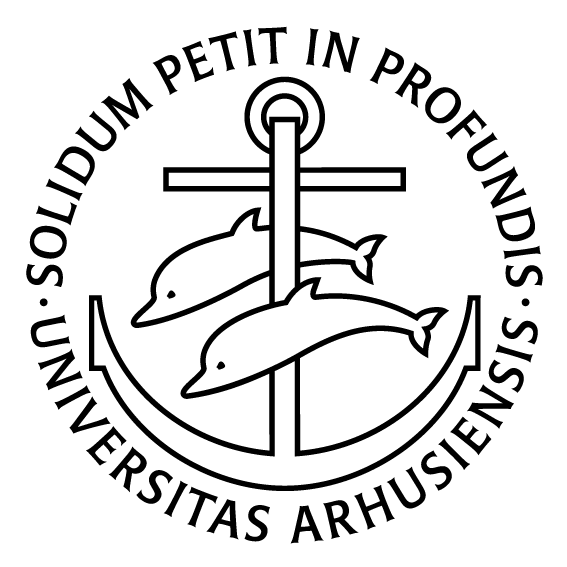
\includegraphics[width=0.5\textwidth]{images/ausegl.png}
        
        \vfill
        \small
        \today
        
    \end{center}
\end{titlepage} % => Display title page

%\tableofcontents % => Display table of contents

\section{Systemskitse udformet som et rigt billede}

\begin{figure}[h]
    \centering
    \includegraphics[width=0.8\textwidth]{images/Systemskitse.png}
    \caption{Systemskitse}
    \label{fig:Systemskitse}
\end{figure} % => Display chapter sections
\section{Systemskitse udformet som et rigt billede}

\begin{figure}[h]
    \centering
    \includegraphics[width=0.8\textwidth]{images/Systemskitse.png}
    \caption{Systemskitse}
    \label{fig:Systemskitse}
\end{figure} % => Display chapter sections
\section{Systemskitse udformet som et rigt billede}

\begin{figure}[h]
    \centering
    \includegraphics[width=0.8\textwidth]{images/Systemskitse.png}
    \caption{Systemskitse}
    \label{fig:Systemskitse}
\end{figure} % => Display chapter sections


%\newpage

\listoffigures % => Display list of figures

\listoftables % => Display list of tables

\printbibliography % => Display bibliography % => Display list of figures, tables and references

\end{document}

